\documentclass{article}
\usepackage[utf8]{inputenc}
\usepackage{xcolor}
\usepackage{amsmath}
\usepackage{amssymb}
\usepackage{graphicx}

\title{Neural Networks Exercise Sheet 1}
\author{Pauline Sander 2581310, Vilém Zouhar 7007410}

\newcommand{\TODO}[1]{{\color{red} TODO: #1}}
\newcommand{\VV}[1]{{\color{blue} Vilda: #1}}
\newcommand{\PP}[1]{{\color{teal} Pauline: #1}}

\begin{document}

\maketitle

\section{Mathematical objects}

The following terms could be defined in an algebraic way. We assume the most common field, $\mathbf{R}$.

\begin{enumerate}
    \item[a)] scalar: single number, $x \in \mathbb{R}$\\
    Example:
    $$
        x'=5
    $$
    
    \item[b)] vector: ordered array, $\textbf{x} \in \mathbb{R}^n, n \in \mathbb{N}$\\
    Example:
    $$
        \textbf{x'}=(4,5)
    $$
    
    \item[c)] matrix: two-dimensional array, $\textbf{A} \in \mathbb{R}^{n\times m}, n, m \in \mathbf{N}$\\
    Example:
        $$
            \textbf{A'} \in \mathbb{R}^{2\times 2}
        $$
        $$
            \textbf{A'} = 
            \begin{bmatrix} 
            5 & 2 \\
            0   & 1\\
            \end{bmatrix}
        $$
        
    \item[d)] tensor: multi-dimensional array, $\mathbf{T} \in \mathbb{R}^\mathbf{v}, \mathbf{v} \in \mathbb{N}^m$\\
    Example:
        $$
            \mathbf{T'} \in \mathbb{R}^{2\times 2 \times 2}
        $$
        $$
            \mathbf{T'}_{1,*,*} =
            \begin{bmatrix} 
            5 & 2 \\
            0   & 1\\
            \end{bmatrix}
        $$
        $$
            \mathbf{T'}_{2,*,*} =
            \begin{bmatrix} 
            1 & 3 \\
            -2 & 5 \\
            \end{bmatrix}
        $$
    
\end{enumerate}

\pagebreak

\section{Vectors in machine learning}

Every datapoint $x$ represents a student and the features are the following:

$$
    \textbf{features} =
    \begin{bmatrix}
        \text{no. finished assignments} \\
        \text{points in the exam} \\
    \end{bmatrix}
$$

Vector representation:
$$
    \textbf{x}_1=
    \begin{bmatrix}
        3 \\
        25 \\
    \end{bmatrix}
$$
$$
    \textbf{x}_2=
    \begin{bmatrix}
        9 \\
        90 \\
    \end{bmatrix}
$$
$$
    \textbf{x}_3=
    \begin{bmatrix}
        7 \\
        53 \\
    \end{bmatrix}
$$
Matrix representation:
$$
    \textbf{X}=
    \begin{bmatrix}
        3 & 25 \\
        9 & 90 \\
        7 & 53 \\
    \end{bmatrix}
$$

\vspace{2cm}
\begin{center}
    \hspace{-2cm}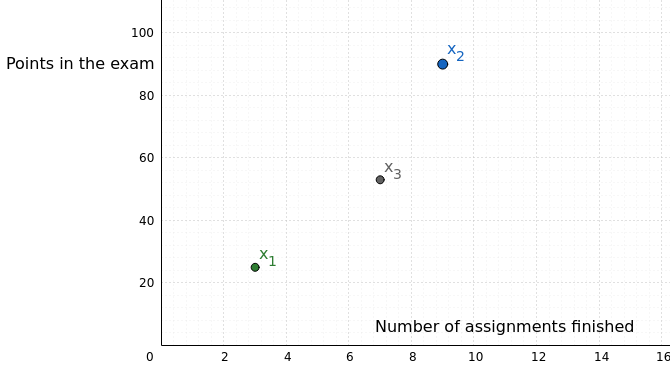
\includegraphics[width=1\linewidth]{img/example_dataset.png}
\end{center}

\pagebreak

\section{Operations on vectors and matrices}

\begin{itemize}
\item[a)]
$$
    \begin{bmatrix} 
    1.5 & 2 & 0.5 \\
    0   & 1 & 1.5 \\
    \end{bmatrix}
$$
\item[b)]
$$
    \begin{bmatrix} 
    15 \\
    17 \\
    \end{bmatrix}
$$
\item[c)]
$$
    \begin{bmatrix} 
    4 & 2 & -9 \\
    -3 & 8 & 0 \\
    \end{bmatrix}
$$
\item[d)]
$$
    \begin{bmatrix} 
    8 & -2 \\
    14 & -4 \\
    \end{bmatrix}
$$
\item[e)] Impossible, because the operation is not defined on the matricies of these dimensions.
\end{itemize}

\section{Multiplication properties, types of matrices}

\subsection{}

\begin{itemize}
\item[a)]
$$
\mathbf{A} \in \mathbf{R}^{n\times m} \text{ is symmetric} \Leftrightarrow \mathbf{A}^T = \mathbf{A}
$$

\item[b)]
$$
\mathbf{A} \in \mathbf{R}^{n\times m} \text{ is orthogonal} \Leftrightarrow \mathbf{A}^T = \mathbf{A}^{-1}
$$

\item[c)]
\begin{align*}
& \mathbf{v} \in \mathbb{R}^n \text{ is a unit vector} \Leftrightarrow |v| = 1\\
& |\cdot|\ \text{is a vector norm}
\end{align*}

\item[d)]
$$
\mathbf{v} \perp \mathbf{u} \Leftrightarrow \mathbf{v} \cdot \mathbf{u} = 0
$$

\end{itemize}

\subsection{}
\begin{itemize}
\item[a)]
$$
(B\lambda I)^T C = \lambda (BI)^T C = \lambda I^T B^T C = \lambda B C \qquad \Rightarrow c), m\times n
$$
\item[b)]
$$
A^{-1}(C A^{-1})^T \lambda = A^{-1} (A^{-1})^T C^T \lambda = A^{-1} A C^T \lambda = IC^T\lambda = C^T \lambda \qquad \Rightarrow a), n\times m
$$
\item[c)]
$$
AA^T B^T C = I B^T C = BC \qquad \Rightarrow c),  m\times n
$$
\end{itemize}

\pagebreak

\section{Vector norms}

$$
|\mathbf{a}|_1 = 6
$$

$$
|\mathbf{a}|_2 = \sqrt{14}
$$

\vspace{1cm}
\begin{minipage}{.44\textwidth}
    \subsection*{a) L1}
    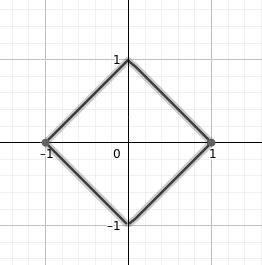
\includegraphics[width=0.8\textwidth]{img/norm_l1.png}
\end{minipage}
\begin{minipage}{.44\textwidth}
    \subsection*{b) L2}
    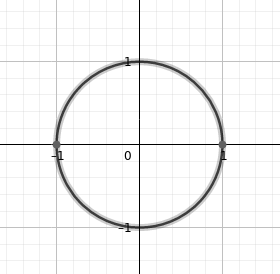
\includegraphics[width=0.8\textwidth]{img/norm_l2.png}
\end{minipage}



\end{document}
